% !TEX root=../../report.tex


\newpage
\Section[angulararchitecture]{Architektur einer Angular Anwendung}

\begin{figure}[h]
\centering
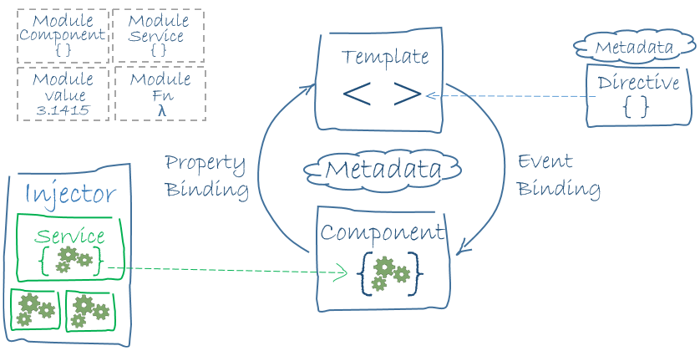
\includegraphics[width=\textwidth]{res/images/overview2.png}
\caption{Architektur einer Angular Anwendung \cite{angularIO}}
\label{aaa}
\end{figure}

Wie in \myautoref{aaa} abgebildet, setzt sich eine Angular Anwendung aus einzelnen Komponenten zusammen. Jede Komponente hat eine eigene Oberfläche und eine eigene Programmlogik. Sie sollen eigenständige, abgeschlossene fachliche Anwendungsfälle abbilden. Die Oberfläche und die Programmlogik sind über Property- und Event-Bindings verbunden. Erstere beschreibt die Bindung aus der Logik in die Oberfläche über Properties. Werden Properties in der Komponente geändert, geben sie die neuen Informationen automatisch an die Oberfläche weiter, wo sie dann angezeigt werden. Letztere beschreiben die Bindung aus der Oberfläche in die Komponente über Events. Diese werden über Aktionen des Benutzers ausgelöst, wie zum Beispiel Eingaben in ein Inputfeld, oder Buttonklicks.

Funktionen, die potentiell wiederverwendet werden können, werden in sogenannte Services gekapselt. Um sie zu verwenden, werden sie über den Injector in die Komponenten injiziert, in welchen die Funktionen benötigt werden.

Zusätzlich werden von Angular vorgefertigte Module bereitgestellt, die für definierte Operationen in die Komponenten importiert werden können. Damit werden Funktionen, wie beispielsweise das Routing, oder auch die Möglichkeit einen \gls{http} Request abzusetzen, behandelt.
